\section{研究背景和动机}
\label{chap:zigzag:motivation}

本章主要介绍研究背景及研究动机,包括基于主动丢包的时间隐通道可行性分析,Zigzag矩阵及其特征,以及CRC数据校验策略三个方面。结合本文\ \nref{chap:backinfo:ctc}对时间隐通道及VoLTE场景的分析,参照本文\ \nref{chap:analyze:result}时间隐通道检测结果,充分利用时间隐通道的构建资源,设计有效的构建方法。

\subsection{基于主动丢包构建时间隐通道}
\label{chap:zigzag:motivation:dropout}
如图\ \nref{fig:2:pmf-dropout},VoLTE网络噪声中,长度为1的离散丢包占据总量的{50\ \%}左右。并且经过本文\ \nref{chap:analyze:result}实验的检验,当时间隐通道的主动丢包率降低到一定程度后,即可规避现有的检测方法。因此,基于主动丢包的时间隐通道,其基本构建原理可行。

对于隐通道双方来说,如何有效定位数据包是一个重要的问题。在VoLTE中,通过RTP头中的Sequence Number字段,即可识别一次通话中的唯一数据包。如图\ \nref{fig:2:rtp-header},数据包序号字段占据{16\ bits},最大可达到65536。正如本文\ \nref{chap:backinfo:rtp:dropout}对RTP丢包处理的描述,丢包后不会出现序号重复的数据包,因此数据包序号满足定位要求。

基于数据包序号构建基于主动丢包的时间隐通道,具有以下优势:
\begin{itemize}
    \item 数据包序号具有传输同步能力,隐通道无需额外的同步时钟,简化了传输流程;
    \item 主动丢包与数据包顺序无关,传输乱序不会影响隐通道;
    \item 主动监听者需要考虑对用户体验的影响,增加丢包或者填充丢包位置均影响通话质量,因此无法完全破坏隐通道;
    \item 即使主动监听者覆写了数据包序号,由于时间戳的线性关系被破坏,接收方能够检测到异常并终止会话。
\end{itemize}

\subsection{Zigzag矩阵及其特征}
\label{chap:zigzag:motivation:zigzag}

\insertFigure{
	\begin{figure}[htbp]
		\centering
        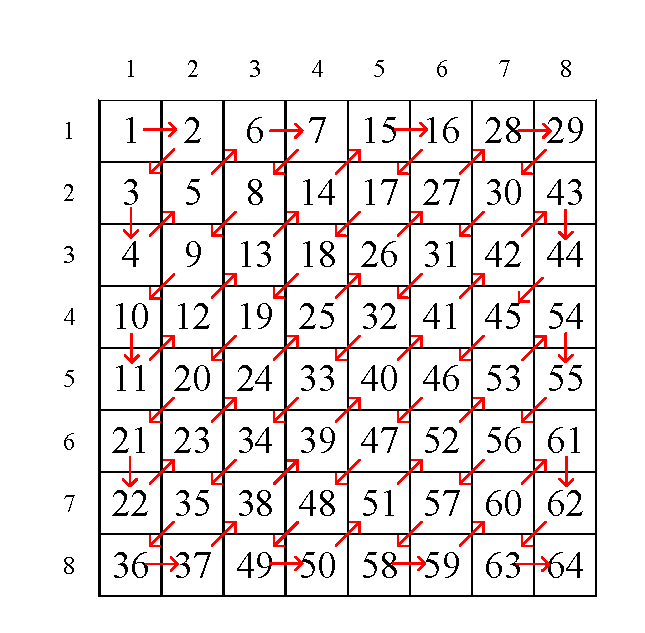
\includegraphics[width=0.5\textwidth]{chapters/chapter4/figures/zigzag-matrix.pdf}
        \caption{8$\times$8的Zigzag矩阵示意图}
        \label{fig:4:zigzag-matrix}
	\end{figure}
}

Zigzag矩阵的排布方式,区别于常见的行优先矩阵或列优先矩阵。由于采用了对角线折返的方式,Zigzag矩阵的坐标与序号无线性关联\nupcite{ji2015a,zaidee2006content,yang2018adaptive,li2019a}。如图\ \nref{fig:4:zigzag-matrix}所示,矩阵中元素的坐标$(x,\ y)$,与元素序号对应。对于$L_{Codeword}=8$的时间隐通道来说,码字按照{4\ bits}切分为前半部及后半部,对应坐标的两个分量$y$与$x$。根据Zigzag映射矩阵的定义,$(C_{4\sim 7},\ C_{0\sim 3})$对应到数据包序号$S$。

另一方面,Zigzag矩阵的起始值支持随机设定,通过起始值初始化能够提高隐通道保密性。即使监听者破解了隐通道的工作模式,并按照相同的方式破解隐蔽消息,在初始化方式未知的情况下破解难度较高。随着矩阵规模的增大,矩阵中元素的排布关系会更加复杂,满足了隐通道的保密性指标。

\subsection{CRC数据校验策略}
\label{chap:zigzag:motivation:crc}

CRC是Cyclic Redundancy Check的缩写,全称为循环冗余校验码,在计算机网络及数据存储中有广泛应用。CRC作为散列函数的一种,可以生成数据的唯一摘要。根据多项式长度的区别,常用的CRC模式为CRC16及CRC32,更多的位数可以保证更低的碰撞概率\nupcite{8736397}。本时间隐通道中,CRC主要用于码字校验,无法利用CRC摘要的全部内容,因此CRC16即可满足校验需求。

\insertFigure{
	\begin{figure}[htbp]
		\centering
        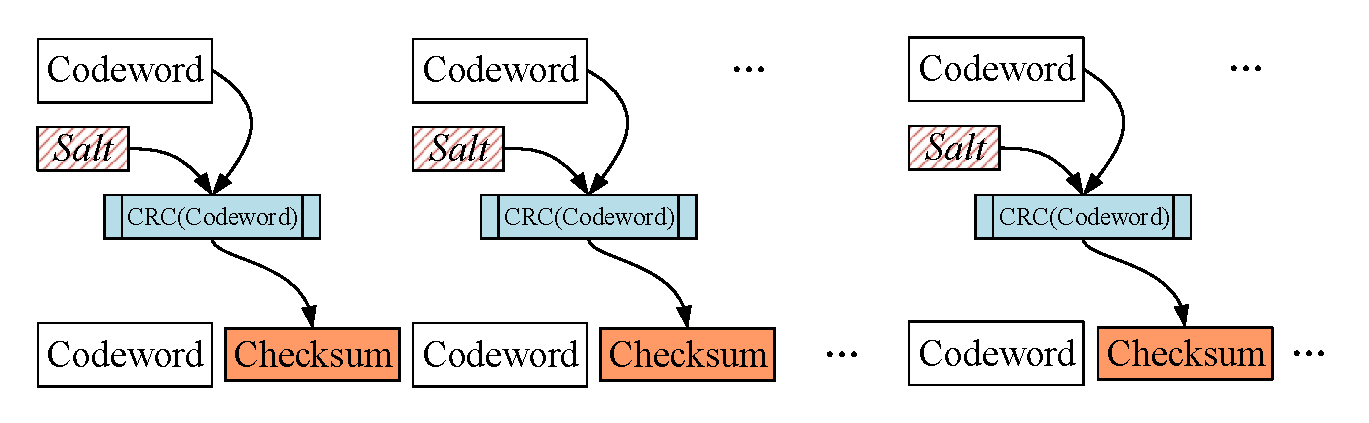
\includegraphics[width=0.9\textwidth]{chapters/chapter4/figures/insert-crc.pdf}
        \caption{CRC校验模式示意图}
        \label{fig:4:insert-crc}
	\end{figure}
}

如图\ \nref{fig:4:insert-crc},数据码字之后追加校验码字,从而通过校验码字区分噪声及信号。CRC函数的源数据,除了当前待验证的码字,还包括$salt$变量,提高计算结果的随机性及保密性。$salt$由两部分组成,一部分是用户共享值$Salt$,一部分是RTP数据包头中导出的随机字段。存在网络噪声的场景中,借助散列函数的单向性,重新验证校验码字筛选数据码字。

\insertTable{
	\begin{table}[htbp]
      \centering
      \caption{添加CRC校验后的码字密度表}
      \label{tab:4:codeword-density}
          \begin{tabular*}{0.98\textwidth}{@{\extracolsep{\fill}}ccccc}
            \toprule
            $L_{Codeword}$ (bits) & $2\times L_{Codeword}$ (bits) & 编码数据包数 & 校验码字编码率 & 总体编码率 \\
            \midrule
            6 & 12 & 128 & 65.6\ \% & 83.6\ \% \\
            7 & 14 & 256 & 66.4\ \% & 82.4\ \% \\
            8 & 16 & 512 & 68.0\ \% & 81.1\ \% \\
            9 & 18 & 1024 & 64.5\ \% & 82.2\ \% \\
            10 & 20 & 2048 & 62.8\ \% & 81.3\ \% \\
            11 & 22 & 4096 & 62.9\ \% & 81.9\ \% \\
            12 & 24 & 8192 & 63.2\ \% & 81.8\ \% \\
            \bottomrule
          \end{tabular*}
    \end{table}
}

组合码字及CRC校验信息,等价于一个超长码字,并且码字中自带校验信息。数据码字及校验码字独立传输的方式,能够有效提高传输效率,保证信道资源的利用率。如表\ \nref{tab:4:codeword-density}所示,传输一个码字,需要$2^{L_{Codeword}}\times 2$个数据包才能完成调制。由于码字位数的限制,CRC摘要的结果只能截取{$L_{Codeword}$\ bits},因此,校验码字存在重复。最终校验码字的编码率在65\ \%左右,总体的编码率在82\ \%左右。

\subsection{研究动机}
\label{chap:zigzag:motivation:conclude}
通过主动丢包的方式构建时间隐通道,最直接的方式是以数据包的相对位置代表隐蔽消息。但在噪声干扰情况下,该模式无法确保鲁棒性。此外,时间隐通道的隐蔽消息通常为敏感信息,即使消息已经加密,隐通道也要保证其安全性。

\insertFigure{
	\begin{figure}[htbp]
		\centering
        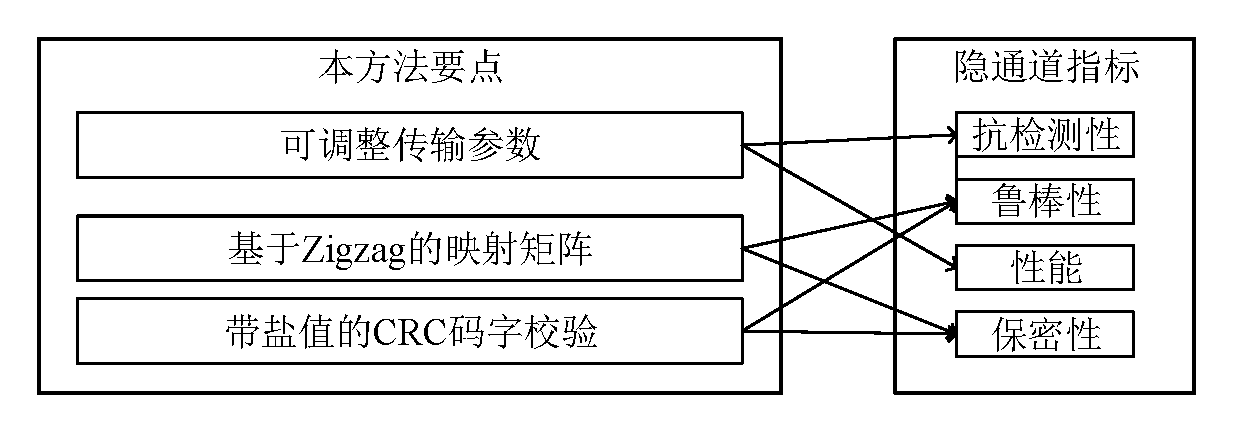
\includegraphics[width=0.8\textwidth]{chapters/chapter4/figures/method-struct.pdf}
        \caption{基于Zigzag映射矩阵的时间隐通道研究要点与指标}
        \label{fig:4:method-struct}
	\end{figure}
}

本章提出的构建方法,通过结合校验码字提高了抗噪声干扰能力。如图\ \nref{fig:4:method-struct},鲁棒性方面基于CRC校验,通过校验信息进行有效数据筛选。抗检测能力方面,传输参数支持不同的$L_{Codeword}$,不同场景中针对配置。保密性方面,引入Zigzag映射矩阵,在码字与符号之间添加转换,并且配合随机初始化增加复杂度;计算CRC校验过程中,添加盐值增强随机性,提高反向破解难度。